\documentclass{paper}
\usepackage[shortlabels]{enumitem}
\usepackage{geometry}
\usepackage{amsmath}
\usepackage{amssymb}
\usepackage{mathrsfs}
\usepackage{graphicx}
\usepackage{float}
\usepackage{listings}
\usepackage{natbib}


\geometry{
  top = 1in
  , bottom = 1in
  , left = 1in
  , right = 1in
  }

\linespread{1.5}
\begin{document}

\title{Potential Changes in Demand Due to Homogeneous Changes in Income and Prices} 
\author{Joshua L. Eubanks}
\bibliographystyle{chicago}

\maketitle
    \begin{abstract}
        % For over a century, fingerprints have been an undisputed
        % personal identifier.  Recent court rulings have sparked
        % interest in verifying unique techniques to make the current
        % methods even more reliable. Ducks, as they do not have
        % fingers, play a key role in the development of new methods to
        % protect the innocent of our society.

        This paper uses intervention analysis to study the effects of the Euro introduction in 2002 to 12 of the 15 members of the EU. In the case of Ireland and Italy, there does not appear to be a significant change in expenditures on food and non-alcoholic beverages after the introduction of the euro. 
    \end{abstract}


\section{Introduction}
The term ``money illusion'' was discussed about 90 years ago when Irving Fisher wrote about it in 1928. His book was more concerned with the common mis-perception of the true value and instability of a currency, rather than a violation of the ``homogeneity postulate'' which was discussed by Leontief 8 years later. It seemed to be a ``catch all'' for many problems in economics such as the non-neutrality of money. Additionally, Dusansky and Kalman argue that homogeneity of degree zero in prices and income is not necessary for demand functions to be free of money illusion and propose a new class of utility functions that are illusion free demand functions (IFDF) which are non homogeneous. \cite{howipati1980b} claim that from an operational viewpoint, however, the homogeneity postulate is reaffirmed since the functions proposed by Dusansky and Kalman fail to examine the properties at the observable points which are the only operationally meaningful ones. Using the homogeneity postulate appears to be best approach to test to see if people suffer from money illusion. 

\subsection{Previous Research}
Much research has been done on this concept. \cite{shafetal1997} conduct surveys posing questions to undergraduates, people shopping at two malls in New Jersey, and individuals at a New Jersey airport on their perception of earnings, transactions, contracts, fairness and morale, and investments given certain questions. This is a good starting point and supports the concept, however, surveys obtain a very skewed sample and people who participate may not necessarily answer questions truthfully and are not sufficiently motivated to. Another experimental design by \cite{fehretal2001} creates a price setting game that would isolate money illusion from other determinants of nominal inertia. They too find money illusion, however, like before, the individual may not necessarily act in the same manner that they would in the ``wild.'' This brings me to a study by \cite{kooretal2004} that seems to fit as a better model of money illusion than the previous ones, since it uses the Euro introduction as a way to see how an individual's perception of money changed. They find a higher rate of donation, but only by percentage changes and do not perform any significance tests since there is no information of the variance of donations. This seems to be a major flaw in to this paper since one could only claim that revenues were higher in one year versus another year. Additionally, they mention that this increase could be due to saving of cognitive effort and divide by 2 rather than by 2.20371 which would support Kahneman's theory in his book \textit{Thinking Fast and Slow} of the ``lazy controller'' in which System 1 (automatic ``knee-jerk'' decision making) overrides System 2 (decision making requiring effort). The ``lazy controller'' is not synonymous with the money illusion concept which is described as a failure to distinguish monetary from real values. Lastly, there is a study about demand functions over time series data in Britain from 54-74 on normal consumption items which finds that demand functions are not homogeneous in prices and income. \citep{deatmuel1980}          

\section{Model}

This will implement the methods used in \cite{cryechan2008}, for the intervention component, and use the final consumption expenditures to predict the level of consumption dollars spent per year on food and non-alcoholic beverages. The idea is to test and see if the expenditures increase/decrease more than what is explained by their changes in income and yearly growth. Additionally, if the effects are significant, I will test to see if the effects are significantly different than the fixed exchange rate to distinguish money illusion from the ``lazy controller'' stated before. Additionally, it would be useful to know the answer to a question such as ``If a US citizen comes to France and 1 Euro is worth 2 dollars, how much more will they spend on food than they would domestically?''

\subsection{Regression Equation}
Implementing an MA(1) process on the curve; where $Y_{t}$ is the total expenditures on food and non-alcoholic beverages in that period, $M_{t}$ is the total expenditures and $T$ is the year.  
$$\log(\hat{Y_{t}}) = \beta_{0} + \beta_{1}M_{t} + \beta_{2}T  + \theta_{t}e_{t-1}$$

 I will follow the notation in textbook written by \cite{cryechan2008} where $m_{t}$ is the change in the mean function due to this shock. I am assuming that this introduction of the Euro gradually dies out and the consumer will return to a consumption pattern similar to before the shock thus, $$m_{t} = \omega_{0}P^{(T)}_{t} + \frac{\omega_{1}}{1-\omega_{2}}P^{(T)}_{t}$$
where $B$ is the backshift operator, T is the time at which the shock occurred, and $P_{t}^{(T)}$ is the pulse dummy variable which is defined as: 
$$
P_{t}^{(T)} =
\begin{cases}
    1, & \text{if } t = T \\
    0, & \text{otherwise }
  \end{cases}
$$
Therefore the final model will look like:
$$\log(\hat{Y_{t}}) = \omega_{0}P^{(T)}_{t} + \frac{\omega_{1}}{1-\omega_{2}}P^{(T)}_{t}+ \beta_{0} + \beta_{1}M_{t} + \beta_{2}T  + \theta_{t}e_{t-1}$$

\subsection{Data}
Choosing the curve allowed me to find the data easier from the UN database for the twelve countries from 1995-2007. I obtained GDP by Type of Expenditure at current prices for final consumption expenditures, and Individual consumption expenditure of households, NPISHs, and general government for expenditures broken down by country and category of consumption. I chose to run the intervention analysis on the two extreme points based off of fixed exchange rates. From \cite{schrsuyk2002} Ireland's exchange rate was 0.787564 Irish pounds per euro, and Italy's was 1936.27 Italian lire per euro. In practice, if money illusion were to exist, they would exist at the two extremes and increase for the case of Italy, and a decrease in the case of Ireland.

\section{Results}
There does not seem to be money illusion after the transition to the euro. Since $\omega$ is not significantly different than zero, there is no reason to see if the ``lazy controller'' effect exists.  

I find the coefficients and standard errors for the covariates as follows for Ireland:

\begin{center}
\begin{tabular}{ c c c c c c c}
 $\theta$ & $\beta_{0}$ & $\beta_{1}$ & $\beta_{2}$ & $\omega_{0}$ & $\omega_{1}$ & $\omega_{2}$\\
 0.5499   &  42.9197    &   0.7140    & -0.0191    & -2.3518  &   -0.0059 & 2.3512\\
 (0.2373) &  (47.6617)  &   (0.2773)  & (0.0273)   & (32.9375)&    (0.0827)& (32.9389)
\end{tabular}\\
$\sigma^2$ estimated as 0.0005439:  log likelihood = 30.23,  aic = -46.47

\end{center}


For Italy:


\begin{center}
\begin{tabular}{ c c c c c c c}
 $\theta$ & $\beta_{0}$ & $\beta_{1}$ & $\beta_{2}$ & $\omega_{0}$ & $\omega_{1}$ & $\omega_{2}$\\

 -0.9968  & -19.1150    &  0.1141     & 0.0207     & -0.0037  &    1.0493 & 0.0154\\
  (0.1998) &  (3.4871)     & (0.0607)      & (0.0026)     & (0.0039)   &   (0.0190) & (0.0009)
\end{tabular}\\

\indent $\sigma^2$ estimated as 8.519e-06:  log likelihood = 56.13,  aic = -98.26\\

\end{center}

It is clear that there is no effect to consumption after the introduction of the euro. For the series of plots below; the top left is an acf, the top right is the pacf (both are before accounting for the changes due to year and income), third is the trend with the points fitted by the MA(1) process. The last plot is, if the effects were statistically significant, the effect of the introduction of the euro in terms of changes to the average consumption.
\begin{figure}[H]
\centering
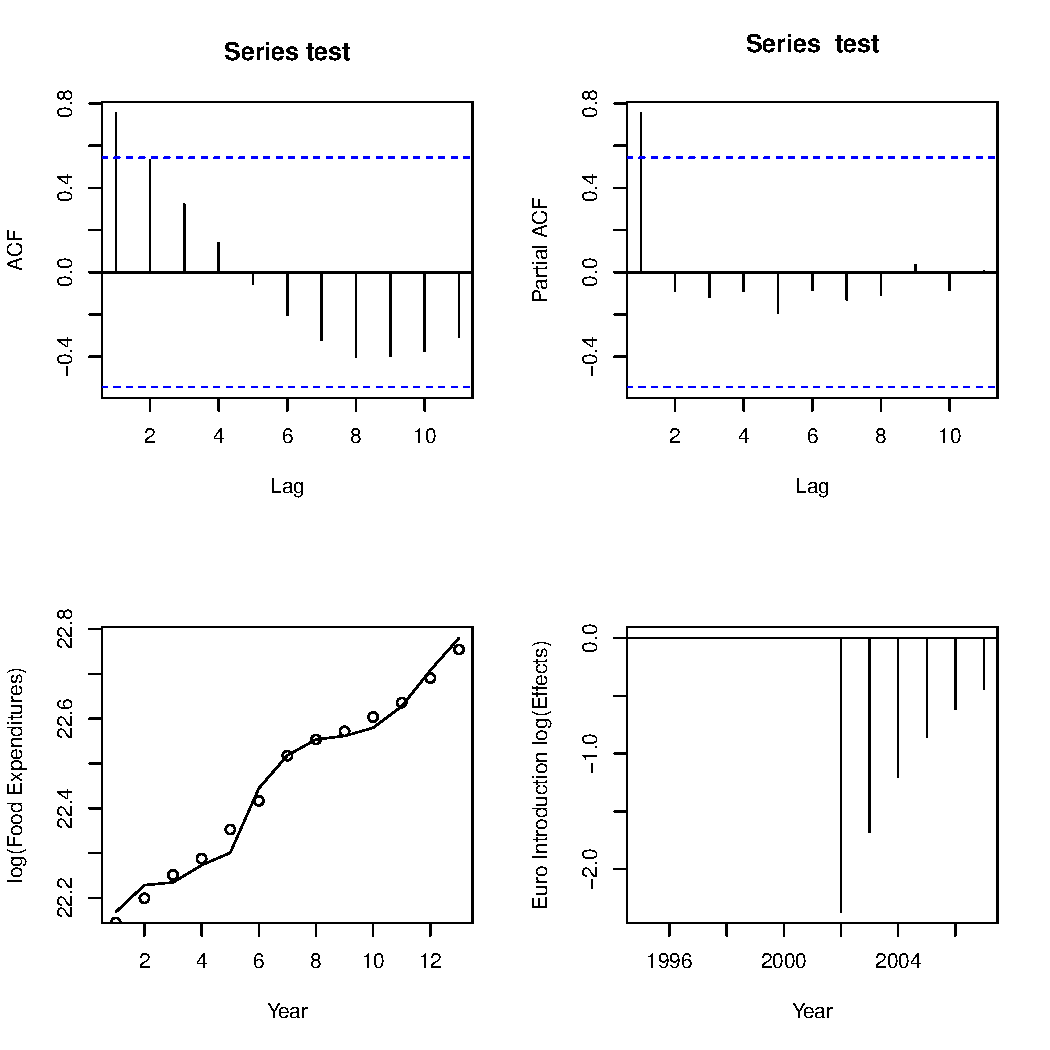
\includegraphics[width = 0.6\textwidth]{Ireland.pdf}
\caption{Ireland}
\end{figure}
\begin{figure}[H]
\centering
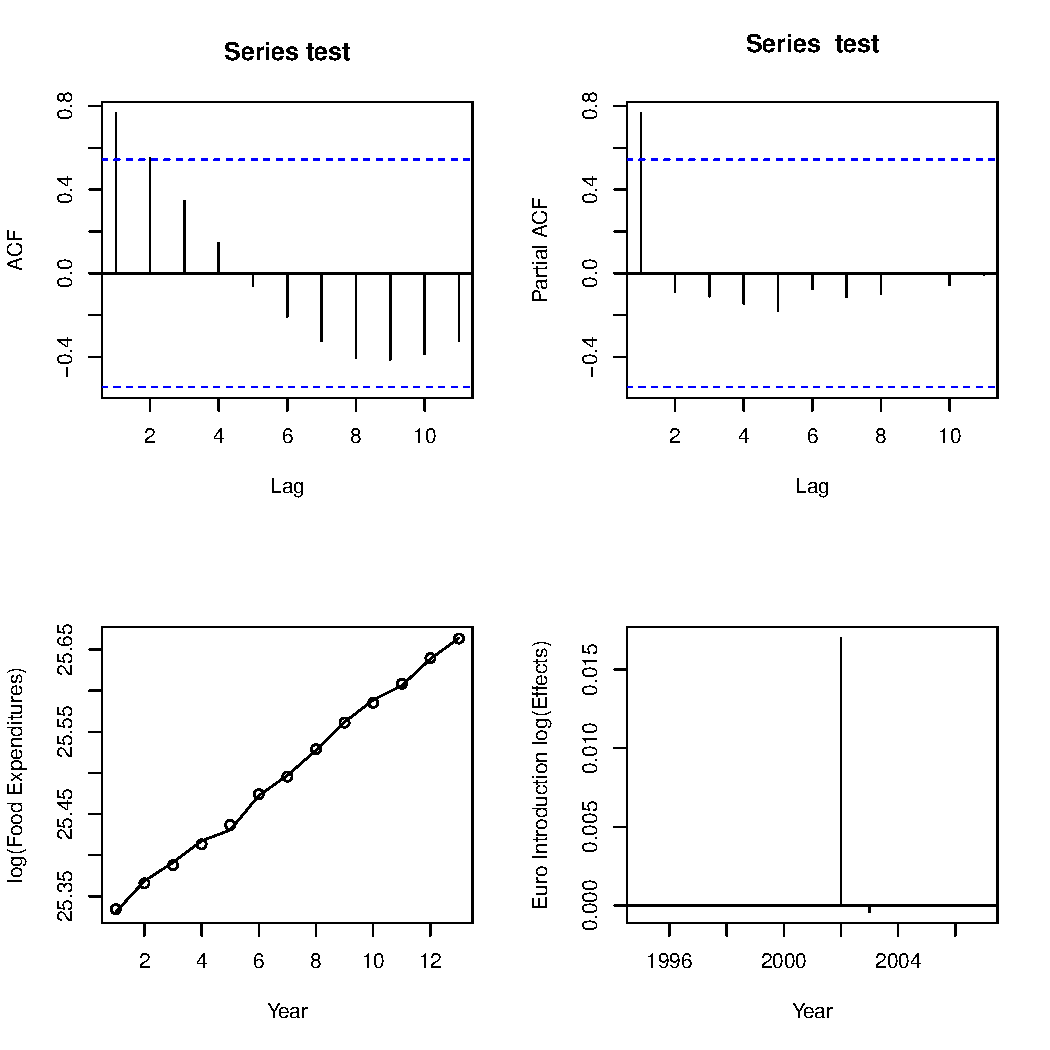
\includegraphics[width = 0.6\textwidth]{Italy.pdf}
\caption{Italy}
\end{figure}
\section{Conclusion}

In the case of normal goods, there does not seem to be an effect from the euro introduction on the consumption pattern of individuals. This, as \cite{kooretal2004} state, is a ``Quasi-Experimental'' design intended to isolate the effect of money illusion. In this case, we should have seen that the Irish consumed less if they acted as \cite{angner2016} claims, to wit, they would believe that one pound for a cup of coffee strikes them as a better deal than 1.5 euros. The converse would be true for Italy in which 1 Euro would appear to be a better deal than 1936.27 lire so they would want to consume more. This however didn't show up in the results. 
\subsection{Discussion} 
In retrospect, it would have been better to find data that was more granular than yearly. Those money illusion effects may have existed at the beginning, and, died out within a few months which would not show in the yearly dataset. Additionally, it would have been preferred to do a study using a demand equation similar to the model presented by \cite{deatmuel1980} since in this case, I am implying that an individual is breaking the homogeneity postulate if they spend a higher/lower proportion than their trend. Unfortunately, the data needed for that kind of study was not as easily accessible such as quantity consumed of butter and the prices of complements/substitutes for all 12 countries. One could further this research and investigate the demand for inferior goods as well, and see if the effect exists in the opposite direction. I am skeptical of my results since I have received different results than what others have, in particular in \cite{deatmuel1980}, they found that demand functions were not homogeneous of degree zero in their study without intervention analysis. My results should have reinforced their results, as a result, I am going to investigate this phenomenon more in the future. 

\bibliography{References}

\nocite{kahneman2011}
\end{document}